\section{Custom Pod Deployer}
Virtual-kubelet \cite{virtual} is an open source project by Microsoft that provides a programmable kubelet API interface to developers. It was developed to run workloads on Container as a Service providers, such as Azure Container Instances. When started with a valid kubeconfig file, Virtual-kubelet registers itself as a node to the Kubernetes cluster and executes commands given from the cluster. It has a programmable backend, called provider, through a Golang interface for developers to write custom deployment logic to their own infrastructure. In Azure's case, using virtual-kubelet, they are registering their container service as a node with almost unlimited capacity, as Azure Container Instances, in theory, can scale up large number of containers without any restriction from the underlying hardware. A shortcoming of that implementation is that those containers can't communicate with the internal Kubernetes services and can't use Kubernetes' load balancing. There are also third-party providers, e.g. AWS fargate or Nomad, to offload workload to their respective container services. Microsoft also uses this techology to connect its Kubernetes service with its Azure IoT Hub service \cite{Chandra2019}. They are deploying Docker containers to their edge devices through the Kubernetes API.

A single Virtual-kubelet instance is started with the following command:
\begin{code}[htpb]
  \centering
  \begin{tabular}{c}
    \begin{lstlisting}[language=python]
      $ ./virtual-kubelet --nodename $ID --provider unikernel --kubeconfig kubeconfig.yaml --labels $LABELS
      \end{lstlisting}
\end{tabular}
\caption{Command to run Virtual Kubelet}\label{lst:vkcommand}
\end{code}


In the command \textit{\$ID} is a random generated string to give as node name. As virtual-kubelet can work with different providers, name of the provider is also given as an argument. The provider written for this thesis is called \textbf{unikernel} and will be explained more in detail. \textit{\$LABELS} sets Kubernetes node labels and it plays a big role on identifying different devices, thus multiple labels can be given.

While developing with Virtual-kubelet a side product of that effort was the ability to simulate large-scale clusters within a reasonable budget. That part is explained in the next section.
\subsection{Simulating Large-scale Clusters}
The working principle of Virtual-kubelet is shown in figure \ref{fig:vk}. As virtual-kubelet is only a binary, it can run in a Docker container and that Docker container can be deployed to the same Kubernetes cluster. It uses the internal kubeconfig file to register itself as a node. Those pods can be scaled to add new nodes to the Kubernetes cluster without scaling up the underlying hardware node count. This creates a testbed for researchers to test new scheduling algorithms. As every node can be given an arbitrary resource value from outside, different resource optimization cases can be tested in an artificially created mega cluster. A pod deployed to a virtual node does not need to run and can be shown as healthy when queried by the Kubernetes master. The only workload that needs to be run is the virtual-kubelet binary, which only takes 34.3 MB in an alpine image when compressed with golang strip flags and upx. A fairly powerful single node Kubernetes cluster can run hundreds of it, and the user will see a 100+ node cluster.

\begin{figure}[htpb]
  \centering
  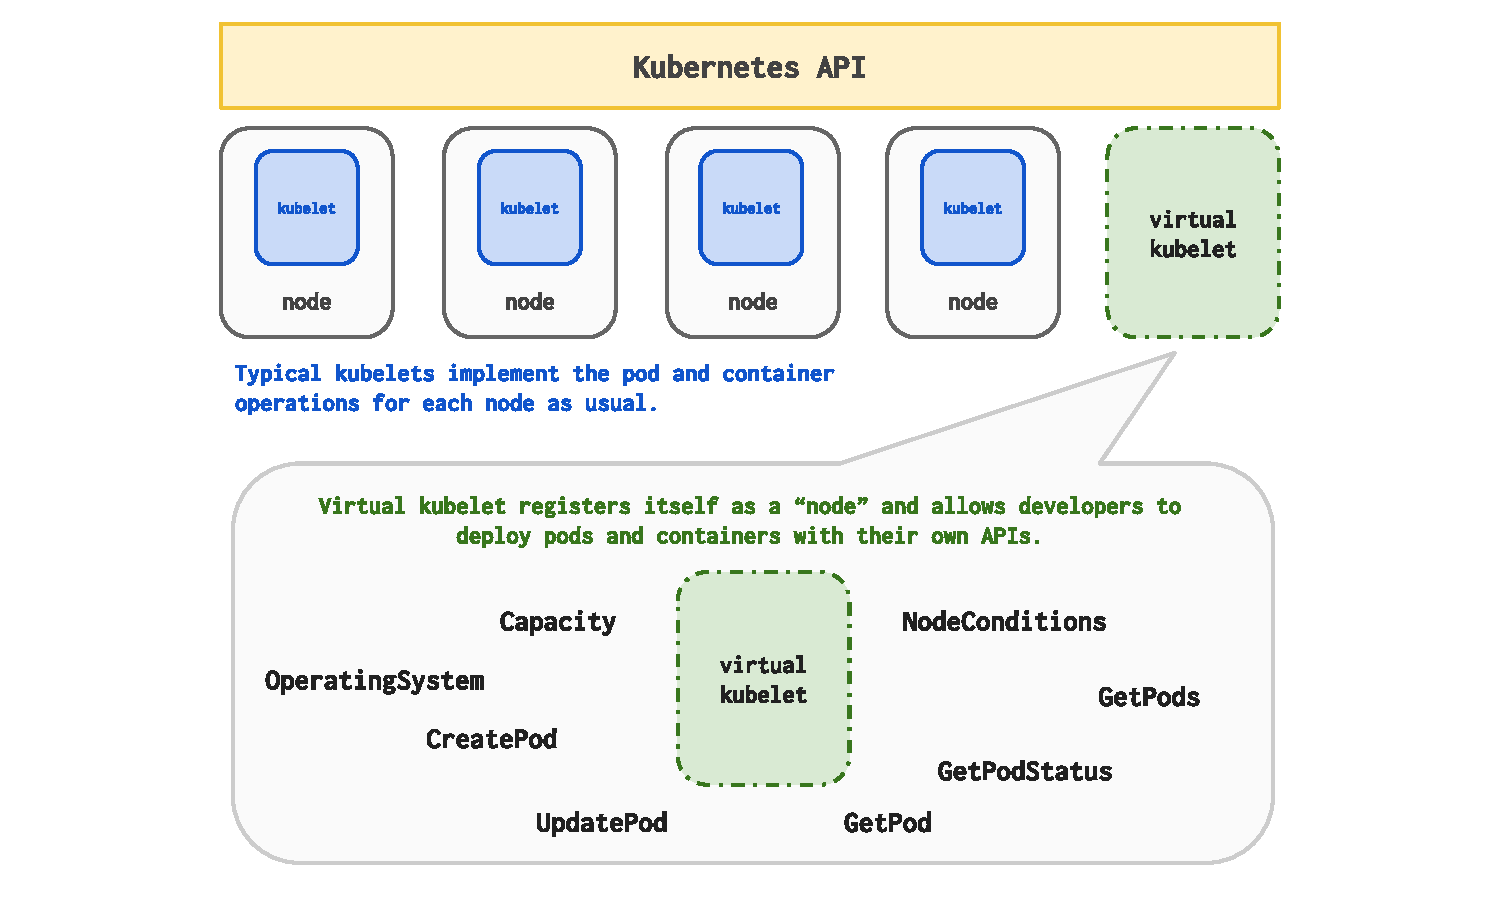
\includegraphics[width=1\textwidth]{figures/diagram.pdf}
  \caption{Working principle of virtual-kubelet \cite{virtual}} \label{fig:vk}
\end{figure}

Another option is to run those containers in a different virtual machine which is not a node of the target Kubernetes cluster. A valid kubeconfig can be used among running containers through a shared volume and a tool like Docker-compose can be used to scale them at will. A chunk of the Docker-compose file can be seen in \ref{fig:docker-compose}.

\begin{code}[htpb]
  \centering
  \begin{tabular}{c}
  \begin{lstlisting}[language=ruby]
    services:
    node-temp:
      build: .
      image: atakanyenel/vk-client
      deploy:
        replicas: 2
      volumes:
        - ${PWD}:/tmp
      environment:
        - LABELS=sensor=temperature
\end{lstlisting}
\end{tabular}
\caption{A virtual node deployment}\label{fig:docker-compose}
\end{code}


A valid kubeconfig file can be found in the same directory as the Docker-compose file and started containers use it to register themselves. When started, this configuration adds two additional nodes to the cluster with the label \textit{sensor=temperature}.

When creating virtual nodes, it's better to use Docker containers, because virtual-kubelet binary listens on certain ports when running and it's hard to start two instances of it on the same machine. Docker containers provide that abstraction.

While testing for this thesis, end devices were simulated on different virtual machines. As It's impossible to setup 100+ devices on the wild, nodes named Rpi-\{random-id\} were generated with different labels according to their simulated tasks.

\subsection{The Unikernel Provider}
The only customizable part of virtual-kubelet is the provider interface. The interface consists of 15 methods that needs to be implemented by the provider developer. Most of the methods are regarding the lifecycle of a pod, while some of them are responsible for the health of the node. 

This thesis implements a single provider called \textit{unikernel} for the unikernel runtime. A single virtual-kubelet binary can support multiple providers through command line arguments as can be seen from listing \ref{lst:vkcommand}. In this project, unikernel deployment is happening in 3 different environments. It's possible to write different providers for different environments but to decrease the built binary size, as all providers are built into the binary, a single provider was compiled using Golang's build tags for different environments. This requires the deployment medium to be known beforehand, instead of virtual-kubelet figuring it by itself by checking the installed hypervisor.

Current open source distribution of virtual-kubelet does not support giving labels to registered nodes. Label based scheduling is an easy way of deploying correct programs to correct end devices, so virtual-kubelet source code had to be forked and modified to update node labels from outside with arguments.

\begin{code}[htpb]
  \centering
  \begin{tabular}{c}
  \begin{lstlisting}[language=go]
import "runtime"
(...)
var m runtime.MemStats
runtime.ReadMemStats(&m)
cpu := strconv.Itoa(runtime.NumCPU()),
memory := strconv.Itoa(int(m.Sys/1024/1024)) + "Mi"

\end{lstlisting}
\end{tabular}
\caption{Getting Resource data}\label{fig:runtime}
\end{code}

The first job done by the provider is to register the resources to the Kubernetes master as available. In the code block \ref{fig:runtime}, the provider constructor reads CPU and memory data from the device where virtual-kubelet is deployed. Kubernetes API uses standartised metrics for measuring CPU and memory, so read values are cast to string before being sent. There is also a third value called \textit{podCapacity}, which restricts the maximum number of pods that can be run on the device, independent from whether the device has enough resources or not.
% Golang Code block start

% Golang Code block end


The following list explains how other functions were implemented in unikernel and hypervisor context. All the functions have a signature similar to DeletePod function in listing \ref{fig:signature}.

\begin{code}[htpb]
  \centering
  \begin{tabular}{c}
  \begin{lstlisting}[language=go]
    func (s *Provider) DeletePod(ctx context.Context, pod *v1.Pod) error
\end{lstlisting}
\end{tabular}
\caption{DeletePod function Signature}\label{fig:signature}
\end{code}


\begin{description}
  \item  [Constructor] runs once and registers the node to cluster. It reads values with code block in \ref{fig:runtime}.
  \item [CreatePod] creates a pod with given pod information from the deployment yaml. All values can be read within the pod object. It calls an \textit{Execute} method, which runs the shell command to invoke the hypervisor with given parameters and returns the context information of the command. This information is saved to an in-memory map with pod name for further reference.
  \item [UpdatePod] updates the unikernel context in memory but not the running process. It's not possible to change parameters of running machines in Xen until next restart, so processes keep running instead of restarting them.
  \item [DeletePod] calls \textit{xl destroy <pod-name>} command to destroy the running unikernel. If the process is not a unikernel and a normal binary, it invokes the \textit{cancel} command which is saved with pod metadata.
  \item [GetPod] returns metadata about the pod from the in-memory map.
  \item [GetPodStatus] calls \textit{GetPod} and returns the status section from metadata.
  \item [GetPods] calls \textit{xl list -l} to get current hypervisor info and parses the json output, updates the in-memory map and returns it.
  \item [GetContainerLogs] finds the command context from the map and returns It's stdout pipe.
  \item [RunInContainer] is no-op.
  \item [nodeAddresses] is no-op but it's possible to return an IPv6 address in the future.
  \item [nodeDaemonEndpoints] returns a default value.
  \item [notifyPods] is no-op.
  \item [capacity] returns values set up with \ref{fig:runtime}.
  \item [ConfigureNode] is only called once. It's set up node information such as the running operating system, processor architecture, addresses, etc.
  \item [nodeConditions] is called periodically to check on node. By checking the remaining capacity on the node, it might return one of the errors: \textit{OutofDisk}, \textit{MemoryPressure}, \textit{DiskPressure}, \textit{NetworkUnavailable}. Because this code is running periodically, developer can write custom functions to check their device for the mentioned errors.
  \end{description}
\subsection{Communication between cluster and device}
Once a virtual node is deployed to the cluster, it is crucial to restrict it to deployments it's supposed to handle. To achieve this, deployments regarding the Virtual-kubelet are tagged with a special label. First the \textit{nodeSelector} array of the specification get the item \textit{type: virtual-kubelet}. With that annotation, no real node tries to handle the deployment. The second annotation is to get the correct provider. In theory, a cluster can have multiple virtual nodes with different providers suited for different workloads and a deployment has to go to It's respective provider. Adding a \textit{tolerations} flag allows to select a particular provider. A chunk of an example deployment file can be seen in \ref{fig:deployment}.

\begin{code}[htpb]
  \centering
  \begin{tabular}{c}
  \begin{lstlisting}[language=python]
    (...)
    nodeSelector:
      type: virtual-kubelet
    tolerations:
    - key: "virtual-kubelet.io/provider"
      operator: "Equal"
      value: "unikernel"
      effect: "NoSchedule"
\end{lstlisting}
\end{tabular}
\caption{Node specific Deployment}\label{fig:deployment}
\end{code}
\textit{NoSchedule} effect protects real deployments from being handled by a virtual node. A pod without the exact tolerations will not be deployed to the node. It's easy to see that all that annotations work both ways. To isolate normal Docker based deployments from virtual nodes and to isolate unikernel based deployments from real nodes.

Another approach of working with unikernel specific deployments is to extend the Kubernetes API by defining a \textit{custom resource}. Custom resources are more handcrafted, because they only contain information given by the developer. Stated by the Kubernetes API, "When you combine a custom resource with a custom controller, custom resources provide a true declarative API." Kubernetes has an Operator Pattern to extend the API in a more official way. In the first development iteration of the Operator Pattern, it turned out that the custom controller would only read data from the \textit{unikernel custom resource} and create a deployment configuration with the labels explained above and the information from the custom resource. Then, that deployment would be handled exactly the same, so it only saves the user from adding above mentioned keys but increases the complexity of the cluster greatly by adding a custom resource definition and a controller.

\tikzstyle{decision} = [diamond, draw, fill=blue!20, 
    text width=4.5em, text badly centered, node distance=3cm, inner sep=0pt]
\tikzstyle{block} = [rectangle, draw, fill=blue!20, 
    text width=5em, text centered, rounded corners, minimum height=4em]
\tikzstyle{line} = [draw, -latex']
\tikzstyle{cloud} = [draw, ellipse,fill=red!20, node distance=3cm,
    minimum height=2em]
  \begin{figure}[!h]
    \centering
\begin{tikzpicture}[node distance = 2cm,auto]
  \centering
  \node [block] (deployment) {Deploy};
  \node [decision,below of=deployment] (schedule) {Has \textbf{effect: NoSchedule?}};
  \node [block,left of=schedule, node distance=5cm] (normal) {Handled by normal nodes.};
  \node [decision,below of=schedule,node distance=5cm] (virtual-kubelet) {Has \textbf{type: virtual-kubelet?}};
  \node [cloud,left of=virtual-kubelet,node distance=5cm] (invalid) {Invalid Configuration};
  \node [decision,below of=virtual-kubelet,node distance=5cm] (provider) {Has \textbf{provider: unikernel?}};
  \node [block,left of=provider,node distance=5cm] (different) {Go to respective provider.};
  \node [block,right of=provider,node distance=5cm] (end) {Handled by Xen.};
  % Draw edges
  \path [line] (deployment) -- (schedule);
  \path [line] (schedule) -- node {no} (normal);
  \path [line] (schedule) -- node {yes}(virtual-kubelet);
  \path [line] (virtual-kubelet) -- node {no} (invalid);
  \path [line] (virtual-kubelet) -- node {yes} (provider);
  \path [line] (provider) -- node {no} (different);
  \path [line] (provider) -- node {yes} (end);
\end{tikzpicture}
\caption{Decision flowchart for unikernel Deployments}
\label{fig:deployment-flowchart}
\end{figure}
\subsection{Communication between virtual-kubelet and hypervisor}
Once a unikernel-specific deployment reaches virtual-kubelet, all of its data can be read. Every method that handles the pod lifecycle has a pod object as argument. This was already mentioned in listing \ref{fig:signature}. The usability of this interface increases greatly when one realises that this pod related information is not read or processed anywhere else other than the running node. It allows to redefine what those values stand for without comprimising the integrity of the system. In a normal pod deployment, the \textit{image} key is used to specify the name of the Docker container that deployment runs. If that container is not found in the given registry, Kubernetes returns an error saying that deployment failed and image couldn't be found. In the unikernel deployment, the image key is used to specify the name of the unikernel binary to run. That name can be handled in many ways. In earlier developments, Docker containers simulating end devices were created with multiple example unikernel binaries, and there were only couple of options to give to \textit{image} key. Now a unikernel registry exists behind a FTP server and given values are searched there first, if they don't exist on the end device. This approach is similar to one used by Docker-based deployments.

\textit{CreatePod} method is responsible for creating new pods. Upon receiving a new pod and checking that pod is valid, this  executes a shell command to talk with the underlying hardware. The shell command executes domain-specific command with supplied parameters. The command runs in a subroutine, and status of the pod is updated as running. While specific commands will be explained more in the upcoming section, an interesting takeaway of this section is how the system does context management with those commands. The binaries are all now running, and if they end up stopping for a reason, they have to be restarted by Kubernetes.

\textit{GetPods} method is periodically called by the Kubernetes API and that method calls another shell command to check started unikernels. For the Xen hypervisor, the output of that command can ben seen in \ref{fig:xenoutput}. That output is parsed as a pod object and returned back to master. The pods are saved in a dictionary with their name as key, and the context of their respective command as value. Their command context allows the system to call the \textit{cancel} closure of a command if that pod needs to be deleted. Their command output can be sent to the \textit{GetLogs} command to return binary output. Golang is very helpful in that area, because by design it has great mechanics for context aware concurrency. The implementation can be seen in \ref{fig:podmetadata}.
\begin{code}[htpb]
  \centering
  \begin{tabular}{c}
  \begin{lstlisting}[language=go]
    type PodWithCancel struct {
      pod        *v1.Pod // v1 "k8s.io/api/core/v1"
      cancelFunc context.CancelFunc // to stop running pods
      output     func() (io.ReadCloser, error) // to read logs
    }
    var pods map[string]*PodWithCancel
\end{lstlisting}
\end{tabular}
\caption{Storing pod metadata}\label{fig:podmetadata}
\end{code}

\begin{code}[!h]
  \centering
  \begin{tabular}{c}
  \begin{lstlisting}
    (...)
    "domid": 1,
    "config": {
        "c_info": {
            "type": "hvm",
            "name": "unikernelapp",
            "uuid": "76d164d3-0201-49c2-9324-4e8e58543b04",
            "run_hotplug_scripts": "True"
        },
        "b_info": {
            "max_memkb": 262144,
            "target_memkb": 262144,
            "video_memkb": 8192,
            "shadow_memkb": 2048,
            "sched_params": {
                "sched": "credit",
                "weight": 256,
                "cap": 0
            },
      (...)
\end{lstlisting}
\end{tabular}
\caption{Xen cli output}\label{fig:xenoutput}
\end{code}



\textit{nodeConditions} is also a periodically called function by the master and it can be configured to reflect changes on the host system. For example, if many unikernel images are running on device, there might be not enough memory to start more instances and that methods would change \textit{OutOfDisk} condition to true.

\pagebreak
When a node disconnects from the Kubernetes cluster, Kubernetes does not re-deploy pods running on it until 5 minutes. The node shows up as NotReady but the pods are still running on it. This is an unwanted scenario for this use case, thus an additional container is deployed to the cluster to delete nodes when they disconnect. That deployment is called \textit{nodeWatcher}. It listens for events regarding nodes, and when a node disconnects, which has the \textit{virtual-kubelet} label, they are also deleted from the cluster. This allows cluster to redeploy pods running on the node without any delay. \textit{NodeWatcher} is a simple container written in python, without any complex logic. It can be used in other scenarios where rapid reaction to node disconnections are desired.